\section{Desarrollo}
{
    \begin{section-definition}[\textbf{División con resto}]
        Para todo polinomio $F$ y $G$ existen los polinomios $Q$ y $R$ tal que
        \[F(x) = G(x)Q(x) + R(x), \quad\mbox{con }  0 \leq \deg{(R)} < \deg{(G)}.\]
        Donde $Q$ y $R$ son el \emph{cociente} y \emph{resto} (o \emph{residuo}) de la división de $F$ por $G$.
        Si $R(x) = 0$, entonces diremos que $G$ divide a $F$, y lo vamos a denotar como $G(x) \mid F(x)$.
    \end{section-definition }

    Abreviaremos $G(x) \mid F(x)$ como $G \mid F$ ya que al efectuar una división polinómica los polinomios en cuestión deben de tener la misma variable.

    \begin{example}
        Con $F(x) = x^7 - 1$ y $G(x) = x^3 + x + 1$ llegaremos a que
        \[x^7 - 1 = (x^3 + x + 1)(x^4 - x^2 - x + 1) + 2 x^2 - 2.\]
        Aquí $Q(x) = x^4 - x^2 - x + 1$ y $R(x) = 2 x^2 - 2$.
    \end{example}

    \subsection{Método clásico}
    {
        Se recomienda cuando los polinomios a dividir son de una sola variable o para polinomios homogéneos.
        El algoritmo es el siguiente:
        
        \begin{enumerate}
            \item Completar y ordenar los dos polinomios, tanto el divisor como el dividendo.
            \item Dividir el primer término del dividendo por el primer término del divisor para obtener el primer término del cociente.
            \item Multiplicar el divisor con signo cambiado por los términos del cociente y sumar ordenamente el producto obtenido con el dividendo.
            \item Tratar el resto obtenido en el paso anterior como el nuevo dividiendo y repetir los pasos b y c.\footnote{En general, los métodos para la división de polinomios son recursivos.}.
            \item Continuar el proceso hasta que el resto obtenido tenga un grado menor al divisor o bien al obtener cero.
        \end{enumerate}
    }

    \subsection{Método de Horner}
    {
        Se recomienda usar el método de Horner cuando el polinomio divisor es de segundo grado o más y se opera solo con
        los coeficientes de los polinomios ordenados y completos. Los coeficientes se distribuyen en un cuadro como el que sigue:
        \begin{figure}[htb]
            \centering
            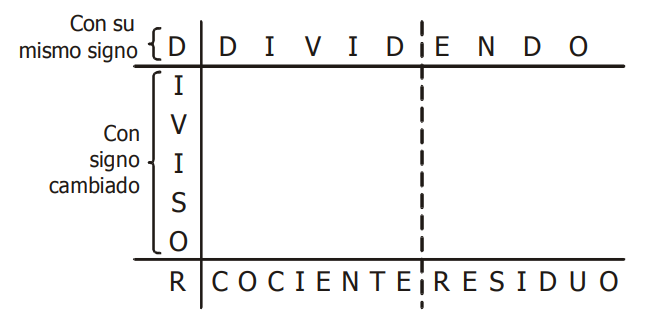
\includegraphics[width=8cm]{images/metodo-de-horner}
        \end{figure}

        Algoritmo del método de Horner
        \begin{enumerate}
            \item Se anotan los coeficientes del dividiendo en la parte superior del cuadro en forma horizontal.
            \item Se anotan los coeficientes del divisor en la parte izquierda del cuadro en forma vertical con los signos cambiados a excepción del primero.
            \item La línea de trazos separa el cociente del resto y para su trazo se considera el grado del divisor.
            En el cociente se cuentan tantos términos como el grado del dividendo menos el grado grado del divisor más uno.
            \item El primer término del cociente se obtiene dividiendo el primer coeficiente del dividendo entre el primer coeficiente del divisor.
            \item El coeficiente obtenido en el paso anterior se multiplica con los demás coeficientes del divisor con signo opuesto y los resultados se escriben en forma horizontal a partir de la siguiente columna hacía la derecha.
            \item Las cantidades que se encuentran en la segundo columna se suman y el resultado se divide entre el primer coeficiente del divisor, repitiéndose el procedimiento hasta coincidir con la última columna del dividendo.
            \item Para finalizar, se suman directamente las columnas correspoindientes al residuo, lo que conformará los coeficientes del polinomio residuo o resto.
        \end{enumerate}
    }
    
    \subsection{Método de Ruffini}
    {
        Se recomienda usar este método cuando el divisor tiene la forma $ax \pm b$. El método de Riffini se considera como un caso particular del método de Horner.
        Este método se apoya de un cuadro como el siguiente
        \begin{figure}[htb]
            \centering
            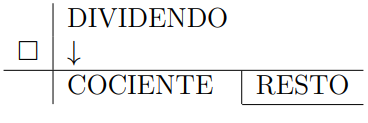
\includegraphics[width=5.5cm]{images/metodo-de-ruffini}
        \end{figure}

        Donde $\boxempty$ es el resultado de resolver la ecuación $ax \pm b = 0$.

        Algoritmo del método de Ruffini
        \begin{enumerate}
            \item Se anotan los coeficientes del dividiendo en forma horizontal y el valor de $\boxempty$ en la columna izquierda.
            \item Se baja el primer coeficiente del dividendo y se multiplica por el valor de $\boxempty$, el resultado se anota en la siguiente columna,
            debajo del segundo coeficiente del dividendo.
            \item Se suman las cantidades de la segunda columna y se sigue el mismo procedimiento hasta obtener un término debajo del último coeficiente del dividendo.
            \item El residuo es la suma de cantidades de la última columna.
        \end{enumerate}
    }

    \subsection{Agregados culturales y preguntas}
    {
        \begin{enumerate}
            \item Existe una rica y abundante literatura sobre la resolución de problemas, entre todas ellas destacamos \textit{El arte de resolver problemas} de \textit{José Luis Córdova}.
            \item He aquí una cita \textit{\("\)En pocas palabras: cualquier problema (por trivial que parezca) lleva a una investigación.
            El gusto por la investigación, la curiosidad, es una de las mayores riquezas de la humanidad.
            Y para investigar no existe ningún camino lógico, sólo el camino de la intuición y la convicción de que existe un orden detrás del caos de percepciones.\("\)}
        \end{enumerate}
    }

    \section{Ejercicios y Problemas}
    {
        Sección de ejercicios y problemas para el autoestudio.
    
        \begin{section-problem}
            Si el polinomio $3x^5 + 6x^3 - 3x$ se le divide entre $x + 1$ se obtiene como resultado un cociente de grado $m$, un término independiente $b$ y un resto $a$. Hallar $m + a + b$.
        \end{section-problem}

        \begin{section-problem}
            Al dividir $x^4 - x^2 - 2x + 1$ entre $x^2 + x + 1$, determine el producto de los términos del cociente.
        \end{section-problem}

        \begin{section-problem}
            Si $P(x - 2) = x^3 - 10x^2 + 28x - 24$, hallar el resto de dividir $P(x)$ por $x - 3$
        \end{section-problem}

        \begin{section-problem}
            Si el resto de la división de $6x^4 - 11x^2 + ax + b$ entre $3x^2 - 3x - 1$ es $3x + 2$. Hallar $a - b$.
        \end{section-problem}

        \begin{section-problem}
            Para que la división de $x^4 + ax^2 + b$ entre $x^2 + x + 1$ sea exacta, encuentre los valores de $a$ y $b$ apropiados.
        \end{section-problem}

        \begin{section-problem}
            Si el polinomio $P(x) = ax^4 + bx^3 + cx^2 + 3x + 1$ se divide por $x^2 - x + 2$ se obtiene un cociente cuya suma de coeficientes es 22 y un resto $R(x) = 10x - 1$, calcular $b + c$.
        \end{section-problem}

        \begin{section-problem}
            Al dividir el polinomio $P(x) = 55x^3 + (166 + b)x - x^2 - 2$ entre $Q(x) = ax^2 - 39x + 2$, el residuo es de la forma $R(x) = mx$. Calcular el valor de $a + b$.
        \end{section-problem}

        \begin{section-problem}
            ¿Qué valor adquire $\dfrac{n + 19}{k + 1}$, si la división $\dfrac{x^{19} - nx + k}{x^2 - 2x + 1}$ es exacta?
        \end{section-problem}
    }
}